\chapter*{Anhang}
\addcontentsline{toc}{chapter}{Anhang}
\section*{Anhangverzeichnis}
\vspace{-8em}

% vor \listofanhang müssen Einrückungen angepasst werden
\abstaendeanhangverzeichnis

\listofanhang
\clearpage
\spezialkopfzeile{Anhang} % damit in der Kopfzeile das Wort "Anhang" angezeigt wird

% \anhang{So funktioniert's}

% \lstset{language=TeX, % hervorzuhebende Keywords definieren
%   morekeywords={anhang, anhangteil}
% }


% \anhang{Experteninterviews}
% Im folgenden Anhangteil finden sich die transkribierten Experteninterviews, welche in verschiedenen Phasen der Bachelorarbeit geführt wurden.



\interview{Philip A.}{Cloud Solution Architekt}{NCS}{Initiales Anforderunginterview}{22.03.2021}{philipp}

\newcommand{\LF}{\textbf{Lukas F.:}~}
\newcommand{\PA}{\textbf{Philipp A.:}~}

\LF	Herzlich willkommen zum Interview und vielen Dank, dass du dich als Interviewpartner bereit gestellt hast

\PA	 Selbstverständlich.

\LF	Ich habe direkt eine Frage an dich: Was ist deine Rolle innerhalb der SPIRIT und was ist deine Rolle im spezifischen mit Perspektive auf die Referenzarchitekturen, die es zu entwickeln gilt?

\PA	Ich sitze in der Spirit auf dem Posten des Cloud Solution Architects speziell für \ac{AWS}. Diese Rolle fülle ich auch in der Native Cloud Solution aus. Das heißt, ich bin für Software und Infrastruktur Struktur Architekturen in dem Projekt/der Solution verantwortlich und kümmere mich darum, dass die Implementierung so gut wie möglich voran gehen kann. Dabei sollen keine Architekturprobleme verursacht werden. Ansonsten berate ich die Entwicklung  bei technischen Fragen und Implementierungsfragen, die auftreten.

\LF	Wenn wir jetzt speziell Richtung Referenzarchitektur schauen, würdest du dich dann eher als Nutzenden sehen oder eher als jemand, der zwar einen \enquote{Stake} hat, dass es eine gute der Referenz Architektur wird, aber sie nicht konkret anwenden würde?

\PA	 Ich sehe mich auf beiden Seiten. Sowohl als Nutzenden, weil ich werde auf Basis der Referenzarchitekturen unsere Serverless Solutions designen, also die für uns und unsere Kunden. Ich glaube aber auf der anderen Seite auch, dass ich mitwirke an der Ausarbeitung.

\LF	 Verstehe, das ist schon mal aufschlussreich. Insgesamt, wir reden ja über Referenzarchitekturen, wo siehst du denn Anwendungsgebiete? Gibt es konkrete Customer Cases, wo wir jetzt auf Zeitreihendaten speziell schauen, oder gibt es da irgendwelche Gebiete, wo du sagst: \enquote{Oh, da könnte es besonders relevant sein}?

\PA	 Ja natürlich. Der größte/aktuellste Fall bei uns sind tatsächlich Sensordaten und Messdaten im \ac{IIoT} Umfeld, bei denen wir solche Zeitreihendaten immer haben. Aber auch sämtliche Monitoring Daten, die von cloudbasierten Metriken abgezogen werden. Von diesen Metriken gibt es viele.

\LF	So wie ich es verstehe, sowohl interne Anwendungsfälle mit Monitoring als auch Sachen, die für Kunden jetzt direkt relevant sind, wie \ac{IIoT}-/Sensordaten

\PA	 genau

\LF	 Das wären denke ich so die Bereiche, in denen man die Referenz Architekturen anwenden würde/ spezialisieren würde.

\PA	 Da wir uns, in der SPIRIT eben auch mit Applikation Management befassen, ist es eben auch ein internes Thema. Wir wollen selber sehen, wie wir möglichst effizient Architekturen zum Betrieb, also auch zum Monitoring aufbauen können. Gleichzeitig ist es auch ein Kundenthema, weil wir öfters Anfragen kriegen zum Thema \ac{IIoT} Umsetzung/ \ac{IIoT}-Implementierung und deren Folgen, die Auswirkung der Daten.

\LF	Insgesamt, wenn wir an Referenzarchitekturen denken, ich rede davon gleich mal im Plural, weil es aus meiner Sicht schon mal mindestens zwei geben muss, als Artefakt meiner Bachelorarbeit. Wie kompatibel sollen die denn zueinander sein, wenn wir uns vorstellen, es gibt zum Beispiel eine für die Echtzeit Verarbeitung und eine für die Batch-Verarbeitung von Daten? Müssen die austauschbar sein, also von derselben Quelle zum Beispiel \enquote{gefüttert} werden? Oder ist es da okay jeweils recht spezifische Pipelines zu bauen, die  dann programmatisch eingebunden werden müssen, relativ nah am Datenerzeugenden?

\PA	 Ich finde, das ist eine Frage, die die Arbeit beantworten sollte, denn ich kann das aus meiner aktuellen Position schwer abschätzen. Für mich ist es nicht klar, ob es sinnvoller ist individuell, also wenn man dem Erzeuger nahestehend die Daten dort auf ein Format zu bringen, die sich laden lassen, oder ob es sinnvoller ist, die Daten vom Erzeuger zu nehmen und dann in der Referenzarchitektur zu normalisieren und anzugleichen.

\LF	 Ich hatte jetzt nicht unbedingt an Daten direkt gedacht, sondern mehr an die Infrastruktur, die kompatibel sein muss. So dass es am Anfang eine Schnittstelle zum Beispiel geben würde, was eine Art Plug and Play mit beiden Ansätzen ermöglichen würde oder einfach das nur einen Ansatz quasi mit mit einer Customization sozusagen funktioniert?

\PA	Ach so. Zu wünschen wäre es natürlich, wenn wir hinterher nur eine Hauptarchitektur hätten oder möglichst wenig Anpassungen an die Architekturen vornehmen müssen, um die Sachen zu switchen. Das ist natürlich aus der Architektenbrille die schönere Sache. Auf der anderen Seite glaube ich tatsächlich, wenn man sich einmal festgelegt hat auf eine von beiden Arten, dass man dann eh nicht mehr switchen wird. \\
Da muss man sich eben vorher klar werden, welchen Weg man gehen will. Es ist eigentlich völlig valide zu sagen, wenn ich weiß, dass ich Batch Verarbeitung mache, dann habe ich auch genau diese Architektur. Die Anforderung, dass man wechseln muss, ist zu vernachlässigen. Interessanter ist es eher, wenn man sagt ich brauche beides. Womöglich lohnt es sich da, beides zu inkludieren.

\LF	 Zu meiner nächsten Frage: Ich habe dir im Vorfeld zwei Listen zugesendet, wo ich gerne deine Meinung hören würde, wie du die jeweils priorisieren würdest. Zum einen sind das die Qualitätskriterien von Referenzarchitekturen und zum anderen die datenbezogenen Entscheidertypen. Fangen wir am besten mit den Qualitätskriterien an.

\PA	 Genau

\LF	Da hat es ja sieben. Welche würdest du denn relativ weit oben aus deiner Position raus positionieren? Und welche sind von eher nachrangiger Relevanz?

\PA	Ich picke von den sieben mal drei raus und vielleicht kannst du mir zu dem einen oder anderen Punkt noch ein bisschen was erläutern. Der Punkt fünf \enquote{akzeptabel}, da verstehe ich nicht so wirklich, was du damit meinst. Beim  Thema \enquote{wertschöpfend für den Betrieb} versteh ich jetzt auch nicht so, was du damit meinst im Vergleich zur Adressierung der Hauptprobleme. Kannst du das nochmal kurz erläutern?

\LF	\enquote{Wertschöpfend für den Betrieb}: So wie ich den Autor verstehe, mein das, das man einen Wert daraus hat, die Referenzarchitekturen anzuwenden und es sich nicht lohnt von \enquote{scratch} anzufangen.

\PA	 Okay. Wie sieht es mit akzeptabel aus?

\LF	Beim Kriterium \enquote{akzeptabel} verstehe ich den Autor so, dass man sich als jemand mit Fachkenntnissen im Prinzip das anschaut und sagt ja, das kann ich akzeptieren mit meinen Fachkenntnissen und das ist jetzt nicht völlig an den Haaren herbeigezogen. Es ist quasi \enquote{reasonable}.

\PA	Das ist ja hoffentlich jeder Architektur. Wenn man das nicht mal voraussetzen kann, dann muss man eigentlich Punkt fünf als ersten nehmen es muss natürlich logisch, also \enquote{reasonable} sein. Das nächste muss sein, dass es wertschöpfend ist in irgendeiner Weise, denn man macht nichts, was nicht einen Mehrwert darstellt. Wo ich Schwierigkeiten habe, ist mit \enquote{reasonable}  weil \enquote{Adressierung der Hauptprobleme} hängt natürlich mit dem \enquote{reasonable} zusammen.\\
Damit eine Referenzarchitektur wertschöpfend ist, muss sie aber auch verständlich sein. Jetzt ist die Frage, wie breit Verständlichkeit gehen muss. Hier steht eine breitere, heterogene Gruppe. So weit würde ich jetzt nicht gehen. Aber es muss verständlich sein für diejenigen, die die Referenzarchitektur anwenden müssen und da tatsächlich relativ einfach verständlich. Aber wenn das andere nicht gegeben ist, dass sie \enquote{reasonable} ist, oder das die Probleme der Domäne nicht abgebildet werden, hilft sowieso alles nix.

\LF	 Das heißt du würdest tendenziell, dass es akzeptabel ist und die Probleme adressiert vorne anstellen, gefolgt von der Verständlichkeit?

\PA	 Nein, wertschöpfend ist tatsächlich noch Nummer zwei, vielleicht sogar Nummer eins. Wenn es nicht wertschöpfend ist, dann brauche ich das nicht zu machen, dann habe ich nur Papierkrieg. Es muss einen Mehrwert für den Betrieb geben, das ist eigentlich Nummer eins, unser zweites ist, dass es akzeptabel sein muss, in Kombination mit der Problemlösung der Domäne. Dann kommen wir zu Thema Verständlichkeit.

\LF	 Verstehe. Wenn wir übergehen zu den Datenentscheider- oder -nutzungstypen gibt es ja drei Stück.  Die taktischen, die operativen und die strategischen Entscheider. Wo siehst du denn uns am ehesten? Letztendlich ist das ja die Basis dafür, die wir die Daten analysieren wollen, also in welchen Entscheidungshorizont wir agieren und mit welcher Dringlichkeit wir neue Daten brauchen, um Entscheidungen abzuleiten.

\PA	 Wer ist denn wir? Das hängt natürlich davon ab, was das für Daten sind und was der Ziel der Daten sind, beziehungsweise was das Ziel ist. Ist das Ziel Monitoring, dann habe ich da natürlich erst mal eine sehr kurzfristige Datenlage, die ich bewerten muss. Also wenn beispielsweise der Speicherplatz vollläuft, ist das wichtiger. Wenn ich irgendwelche \ac{IIoT} Daten habe, kann es durchaus sein, dass das eher langfristige Informationen sind. Wenn ich die Temperatur messe oder den \coo{} Gehalt messe, habe ich auch durchaus Interesse an der Langfristigkeit der Daten.

\LF	 Verstehe also tendenziell würdest du, wenn es um Monitoringdaten geht eher dem taktischen Entscheidertyp folgen, der recht früh betrachtet, wenn sich was ändert und seine Entscheidung im Zweifelsfall anpasst. \ac{IIoT} siehst du also eher Richtung operative Entscheider?

\PA	Auch da hängt es wieder von der Art der Daten ab. Wenn es ein \ac{IIoT} Sensor ist, der messen soll, ob es ein Feuer gibt, dann ist es eine taktische Entscheidung, dann den Feueralarm zu betätigen. Wenn es aber Daten sind, die das Wetter beobachten, dann ist es vielleicht interessanter als strategischer Entscheider ranzugehen. \\
Es ist sehr datenbezogen. Beim Monitoring vielleicht ein bisschen weniger. Auch aus Monitoringdaten kann ich natürlich Sachen ziehen, wenn ich nach einem halben Jahr Monitoring sehe, in welchen Intervallen meine Systeme besonders ausgelastet sind. Davon können natürlich auch Entscheidungen abgeleitet werden. Die meisten Informationen beim Monitoring sind aber tatsächlich kurzfristige. Und bei \ac{IIoT} kann ich das kann ich das gar nicht einschätzen, weil da bin ich nicht so tief drin und die Systeme von \ac{IIoT} sind so mannigfaltig. Das ist ja keine Domäne an sich, sondern es ist ja eher eine Infrastruktur, die auf verschiedene Domänen anwendbar ist, je nachdem, was das für Sensordaten sind oder auch in welchen Intervallen die abgefragt werden. Wenn es Sensoren gibt, die jede halbe Stunde Daten melden, dann ist die Echtzeit Entscheidung eher sekundär. Wenn es aber Daten sind, die alle zehn Sekunden anfallen, ist das eher interessanter für Echtzeitentscheidungen.

\LF	 Also du meinst es kommt wesentlich auf die Messdistanz der Sensordaten an?

\PA	 auf jeden Fall

\LF	 Verstehe. Zum zweiten Teil des Interviews: Ich habe ein Dimensionsmodell konstruiert für Referenzarchitekturen, wo es jetzt um die subjektive Allgemeingültigkeit, die Anwendbarkeit, und die Dekompositionstiefe gehen soll. Jetzt wäre meine Frage jeweils, wie du drei Punkte einschätzt auf einer Skala von Null bis fünf und wieso. Wie wichtig ist dir subjektive Allgemeingültigkeit, wie tief muss eine Dekomposition stattfinden, damit Referenz Architekturen gut sind und wie konkret oder abstrakt darf die Referenzarchitektur sein, dass sie nutzenstiftend für viele Anwendungfälle ist, aber trotzdem eingesetzt werden kann.

\PA	 Die Allgemeingültigkeit und die Anwendbarkeit hängen stark vom Teilnehmerkreis ab, also wie groß sehen wir den Teilnehmerkreis der Leute, die mit dieser Referenzarchitektur arbeiten sollen? Je größer der ist, desto größer muss natürlich auch die Allgemeingültigkeit sein. Wenn wir das in dem relativ engen Rahmen sehen, auf Abteilungsebene oder vielleicht bisschen größer, dann können diese beiden Punkte relativ eng gefasst sein. \\
Bei der Dekompositionstiefe , das ist aus meiner Sicht eine Fleißarbeit. Je detaillierter die Dekompositionstiefe ist, desto einfacher ist es vermutlich, die Referenz Architektur in eine echte umzusetzen Architektur. Man hat da ja dann schon viele Hilfestellungen, Beispiele, etc. . Erfahrene Architekten können dann auch die Dekompositionstiefe wählen, die sie brauchen. Die Dekompositionstiefe ist bei der Anwendbarkeit Teil des Kontext. Da ist es eben die Frage, wie groß die Bandbreite ist, wenn wir sagen, wir haben genau diese zwei Usecases, nämlich Monitoring und \ac{IIoT}, dann kann die schon relativ konkret sein. Wenn wir sagen, wir haben vor, das irgendwie über die komplette Organisation und Firma zu stülpen, dann ist es halt sehr abstrakt. Ich halte nicht so viel davon, Dinge zu abstrakt zu machen, weil sie dann tatsächlich oft nicht verstanden werden und auch nicht benutzt werden. Je abstrakter ich Sachen mache, desto geringere Dekompositionstiefe habe ich normalerweise. Insofern würde ich die das Thema Allgemeingültigkeit er so im mittleren und unteren Bereich sehen, genauso wie die Anwendbarkeit und Dekompositionstiefe so tief wie möglich.

\LF	Wenn du das auf einer Skala, wo null das schlechteste/geringst abstrakteste etc. ist und fünf die Vollausprägung, also sehr spezifische Allgemeingültigkeit beispielsweise, wo würdest du das dann jeweils sehen?

\PA	 Dann würde ich sagen, die subjektive Allgemeingültigkeit sollte irgendwo bei drei bis vier liegen, genauso die Anwendbarkeit im Kontext und die Dekomposition sollte sehr, sehr tief sein bei fünf.

\LF	 Herzlichen Dank, ich denke das ist für das erste Interview schon recht viel, was ich für meine Arbeit mitnehmen kann. Gerne würde ich mit dir ein weiteres Interview zum Abschluss der Arbeit machen, bei der wir die jetzt erarbeiteten Kriterien auf meine Artefakte anwenden.

\PA	 Können wir so machen.

\LF	Gut, dann vielen Dank für das Interview und deine Zeit.

\PA	 Gerne.
\pagebreak
\anhang{Experteninterview Peter E.}\label{chap:interview-peter-24.03.2021}
\begin{table}[H]
\begin{tabularx}{\textwidth}{|l|X|}
\hline
    Datum                  & 24.03.2021 \\ \hline
    Thema                  & Initiales Anforderungsinterview \\ \hline
    \begin{tabular}[c]{@{}l@{}}Teilnehmende,\\ Position\end{tabular} & \begin{tabular}[c]{@{}l@{}}Lukas Fruntke, Verfasser\\ Peter E., Head of Solution - \ac{IIoT}\end{tabular}\\ \hline
\end{tabularx}
% \caption{Interviewübersicht Peter E.}
% \label{tab:interviewuebersicht-peter-24.03.2021}
\end{table}
\newcommand{\PE}{\textbf{Peter E.:}~}

\LF Hallo Peter, herzlichen Dank dass du dir die Zeit genommen hast mir als Interviewapartner zur Verfügung zu stehen! Kannst du bitte kurz beschreiben, welche Rolle du in der SPIRIT inne hast und wie deine Rolle mit Zeitreihendaten und Referenzarchitekturen zusammenhängt?

\PE Meine Rolle in der SPIRIT ist laut offizieller Bezeichnung Head of Solution \ac{IIoT} und Automation. Das heißt ich kümmere mich um die gesamten \ac{IIoT} Projekte, die in der SPIRIT abgewickelt werden. Sei das Geschäftsentwicklung, Kundenbetreuung, Personalaufbau, Presales, ... oder anderes. Wir beschäftigen uns hauptsächlich mit der Digitalisierung von Städten, z.B. mit der Prozessoptimierung im Energie- und Versorgungsbereich. Dabei digitalisieren wir die ganzen Strom-, Gas-, Wasserzähler und lesen diese via Funk aus. Ich arbeite eigentlich ausschliesslich mit Zeitreihendaten, weil ein typisches Merkmal von \ac{IoT} Projekten ist, dass diese gesammelt und auf verschiedenste Arten ausgewertet werden. 

\LF Verstehe. Das Ziel meiner Bachelorarbeit ist ja, Referenzarchitekturen für die Verarbeitung von Zeitreihendaten in der Cloud, speziell in \ac{AWS} zu konstruieren. Wo siehst du denn Einsatzbereiche für solche Referenzarchitekturen, also Kundencases o.ä.? 

\PE Wir haben eigentlich immer die gleiche Grobarchitektur, nach der die Datenverarbeitung läuft. Im Feld sind Sensoren, die über Gateway Services, welche die Daten in ein einheitliches Format harmonisieren, Daten erfassen. Die Daten kommen dann in ein Backend, wo sie verarbeitet werden und werden abschliessend gespeichert. Vom Speicherort aus werden die Daten momentan weiterverarbeitet. Das ist dabei sowohl Visualisierung als auch Übergabe an z.B. Drittsysteme. 

\LF Wenn man das auf mein Feld, die Cloud überträgt, wäre die Analyse \enquote{hinten raus} ja eine der Möglichkeiten für eine Referenzarchitektur.

\PE Ja, aber du hast ja abgesehen davon auch in der Cloud Services, um dir deine Datenbeschaffung zu ermöglichen, wie z.B. den \AWSIOT Core, also den \ac{MQTT} Broker. An den kann man ja die Gatewayservices anknüpfen. Wenn ich mich richtig erinnere, bietet aber auch \ac{AWS} verwaltete Gatewayservices zur Datennormalisierung an. Letztenendes könnte man diese Architektur also auch komplett in \ac{AWS} abbilden.

\LF Ja das wäre auch ein gute Option, ich denke aber, dass es nur bedingt Sinn macht das in \ac{AWS} nochmal komplett neuzubauen, da ihr ja schon einige laufenden Konverter habt, die die Daten der Sensoren in maschinenlesbare Formate umwandeln. Ausgehend von diesen umgewandelten Daten wäre aus meiner Sicht eine Analyse viel spannender.

\PE Verstehe, da könnte man ja die Daten aus der IoT Plattform ausleiten und Richtung \ac{AWS} senden. Dies tun wir bereits so ähnlich in einem Kundenprojekt via \ac{MQTT}, wo wir die Daten zur TU Dresden für Analysen ausleiten. Wir haben ja aber auch die \coo{} Sensoren in unseren Konferenzräumen, die permanent Daten sammeln, die könnte man ähnlich weiterleiten.

\LF Ja, die \coo Daten hatte ich auch schon im Kopf.

\PE Wenn du Auswertungen aber fahren möchtest, die statistisch belastbar sind, dann brauchst du ja Daten, die häufig und in großer Menge ankommen.

\LF Ja, dafür habe ich den Gerätesimulator entworfen, mit dem ich in einem kurzen Intervall Daten in den \ac{MQTT} Broker bringen kann. 

\PE Wichtig ist, dass du die Usecases nach Datenfluss vergleichst. Also was und wie viel kommt von außen rein und welche Analysen möchtest du drüber fahren? Letztenendes ist das, was du machen möchtest das, was Ralph mit der \ac{IoT} Plattform über Jahre gemacht hat. Das ist auch eine Referenzarchitektur. Da hat er sich überlegt: \enquote{Was könnte man nehmen um Zeitreihendaten zu speichern ?} - da kam er auf Elasticsearch. \enquote{Wie bekomme ich Daten in die Plattform?} - Da ist er nach langer Suche auf \ac{MQTT} gekommen. \enquote{Wie kann man eine Verarbeitungslogik gestalten?} - Da kam er auf Node-Red.

\LF Im Prinzip geht es genau um solche Referenzarchitekturen, die explorativ zu erarbeiten. 

\PE Das erste was du brauchst für die Referenzarchitektur ist eine Datenbank, die große Mengen an Zeitreihendaten verarbeiten kann.

\LF Ja, das ist eine Möglichkeit. Ich möchte mir aber auch Streamingdaten vom Broker direkt anschauen. Für Anwendungsfälle wie Schwellenwerte brauche ich die Daten nicht in der Datenbank, sondern kann schon vorher sagen, ob man einen Alarm auslösen muss.

\PE Ja wobei du bei der Schwellwertanalyse natürlich Karenzzeiten beachten musst. Wenn beispielsweise in einem Kühlhaus ein Temperatursensor vorne an der Tür ist und du einen Alarm auf 0 \textdegree{}C hast. Dann reicht es, wenn die Tür zum Ent- oder Beladen aufgemacht wird, um den Alarm auszulösen. Ohne Karenzzeit hat man hier nen Alarmzustand, mit entsprechender Karenzzeit von beispielsweise 10 Minuten verhindert man solche Fehlauslösung.

\LF Ja, das müsste man aber auch in einer Echtzeitpipeline abbilden können. Generell geht es darum sich die verscheidenen Verarbeitungswege von Daten in \ac{AWS} anzuschauen. 

\PE Okay, dann musst du aber bei der Datenquelle Unterscheidungen treffen. Es gibt zum einen diskrete Daten, wie beispielsweise Zählertelegramme von Wasserzählern. Dieser \enquote{beamt} ein Telegramm raus, in fünf Minuten das nächste und so weiter. Das ist kein kontinuierlicher Strom, sondern der sendet immer ein Datenpaket in einem Zeitabstand $x$. Oder man bekommt Daten von einem Sensor, wenn sich etwas ändert. Das sind keine Streamingdaten, sondern Zeitreihendaten. Ich weiß dabei nicht, ob man kontinuierliche Daten über \ac{MQTT} übermitteln kann.

Es gibt drei verschiedene Datenkategorien. Das eine sind Events. Das heißt die Infrastruktur meldet einen Status oder ein Ereigniss, auf dass dann in einer Infrastruktur reagiert wird. Diese Events sind auch Zeitreihendaten. Wenn wir in die IT schauen, gibt es in einem Server Events, wo beispielsweise übermittelt wird \enquote{Meine Platte ist voll}. Dieses Event wird alle paar Minuten übermittelt, weil es beispielsweise ein Schwellwert ist. Diese Ereignisse enthalten keine Messwerte, sondern sind ein Ergebniss einer Messwertauswertung. Trotzdem laufen sie als Zeitreihendaten ein, weil sie hintereinander kommen, wie Messwerte auch. In einer Auswertung dieser Daten könnte man die dann deduplizieren oder eine Korrelation zu Metadaten machen. Wenn in einem Rechner z.B. die Gehäusetemperatur und die CPU und weiteres zu hoch ist, lässt das auf überhohe Last schliessen. 

Der nächste Typ wäre Metriken, also Messwerte. Aus der Auswertung dieser Werte kann man dann selbst solche Events generieren. Das ist dann aber die Aufgabe der eigenen Auswertungslogik. Messwerte können diskret haben, wenn diese in einem zeitlichen Abstand kommen. 

Es gibt aber auch Sensoren die \enquote{kontinuierliche} Messwerte liefern. Das ist dann Streaming.  Das betrifft nicht nur IoT sondern Automatisierungstechnik generell. Bei diesen drei Arten unterscheidet sich jeweils die Verarbeitung. Gestreamte Messwerte wären beispielsweise, wenn man aneiner stromporduzierenden Windturbine hängt. Dabei misst man in einem relativ engen Zeitraster, wie der Verlauf der Leistungskurve aussieht. Oder man misst, wie die Stromkurve oder die Phasenverschiebung aussieht. Die Daten sind sehr eng zeitlich gerastert, damit man auch kleinste Änderungen mitbekommt. 

\LF Du machst also den Unterschied zwischen diskreten Messwerten und \enquote{Streamingdaten} abhängig von der Messdistanz, weenn ich das richtig verstehe?

\PE Richtig. Im Prinzip kann man sagen, wenn die Daten einen gewissen zeitlichen Abstand unterschreiten, kann man von einem Stream sprechen. 

\LF Generell soll das Ziel der Referenzarchitektur sein, verschiedene Messdistanzen zu erlauben, seien das jetzt Milisekunden oder Minuten.

\PE Genau, und wenn du einen Milisekundenabstand hast, dann bist du sozusagen im Streaming mode. Da muss dann deine Infrastruktur dahinter permanent auf Höhe sein, damit die ja nix verpasst. 

\LF Ja, das ist einer der Punkte wo aus meiner Sicht die Cloud interessant wird.

\PE ja, aber die Cloud wird auch schon bei Daten interessant, wenn ein hohes Volumen von vielen Devices eintrifft. Wenn man beispielsweise eine Stadt nimmt, die Smart Meter breit einsetzt, dann haben die bei einer größeren Stadt über 70.000 Devices verteilt. Die senden dann vielleicht nur alle 15 Minuten ein Messwert. Wenn aber jetzt ein Stromzähler pro Telegram 50 Bytes sendet, alle 15 Minuten und das multipliziert mit 70.000 ist die Cloud schon sehr interessant.

\LF Ja, das sehe ich auch so. Es kommt ja zum einen auf die Menge $n$ der Sensoren an und zum anderen eben auf die Messdistanz.

\PE Genau. Um mal bei dem Windradbeispiel zu bleiben: Ein Windrad kann eine Dateninfrastruktur schon ziemlich unter Stress setzen, wenn man zeitlich enge Raster braucht, weil man kleinste Abweichungen mitbekommen will. Kennst du da aus der Messtechnik das Shannon Theorem? \textit{(Nyquist-Shannon-Abtasttheorem)}

\LF Nein.

\PE Da geht es um Analog-Digital Wandlung. Auf einer Stromleitung hat man ja einen Sinus von 50 Hz. Das ist ja ein kontinuierliches Signal. Wenn man diese Kurve jetzt samplen, also digitalisieren will, möchte man ja eine Art Messpunkt an der Kurve anlegen, um die Sinuskurve in ein zeitlich enges Raster aus digitalen, diskreten Messwerten zu legen. Das Theorem sagt, dass man mindestens  mit der doppelten Messfrequenz so ein Signal abtasten muss, um das richtig herauszubekommen. Also muss ein Analog Digital Wandler mindestens mit 100Hz abtasten. Wenn der Analog-Digital Wandler jetzt eine Auflösung von 16 bit hat, wird die Amplitude der Sinuskurve in $2^{16}$ \enquote{Stifte} zerteilt. Das heißt pro Messample hat man 2 bytes, dann hat man 100 Samples pro Sekunde mal 2, also 200 bytes pro Sekunde, nur bei 50Hz. Bei einem schnelleren Signal muss man das entsprechend schneller abtasten. Normalerweise werden Signale mit der vierfachen Frequenz gesampled, also 200Hz und 200 Datenpunkte pro Sekunde. Das ist dann Streaming. Das kommt immer zum Einsatz, wenn man analoge Signale digitalisiert, wie hier die Spannung, die  ins Netz eingespeist wird.

\LF Auch solche \enquote{Streaming} Usecases sollte meine Architektur unterstützen. Idealerweise skalieren die eingesetzten Dienste ja auch.

\PE Von diesen Lastanforderungen kann man ableiten, welche Dienste man im Hitnergrund von \ac{AWS} braucht, um das zu verarbeiten. Diese Methodik habe ich beim HP in der IT-Datacenterautomatisierung/Überwachung/Monitoring schon gehabt. Das gleiche trifft aber auch so auf \ac{IoT} zu. Das ist auch einer der Gründe, warum man die gleiche Software für IT-Automatisierung und für den Maschinenbau einsetzen kann. Das ist die gleiche Software. Wenn du so eine Referenzarchitektur also erstellt hast, kann man die nicht nur für \ac{IoT} benutzen. Das ist wichtig. Man kann die auch für IT benutzen.

\LF JA, die Idee die Referenzarchitektur auch für Monitoring zu verwenden, die besteht. Ganz viele Daten sind ja Zeitreihendaten.

\PE Der Fakt, dass man solche Systeme sowohl für \ac{IoT} als auch IT verwenden kann, ist für mich ein unique selling point. Das Beispiel dafür ist mein Windparkmanager, den ich beim HP gemacht habe. Da habe ich das andersrum gedreht. Da habe ich die IT-Monitoringsoftware genommen und für \ac{IoT} Geräte verwendet. Die Kunden waren begeistert! 

\LF Verstehe, diese Dual use Möglichkeit werde ich auf jeden Fall nochmal erwähnen in der Bachelorarbeit. Ich hätte auch noch ein paar Fragen vorbereitet. In der Literatur gibt es die Aussage, dass es drei verschiedene Entscheidertypen gibt (Erklärungen siehe \autoref{abb:DataHalflife}). Es gibt taktische, operative und strategische Entscheider. Welche Entscheider findest denn du am wichtigsten?

\PE Die wichtigsten sind aus meiner Sicht die taktischen Entscheider, welche wohl den fachlichen Entscheidern in den Fachabteilungen entsprechen. Diese Leute sitzen im operativen Geschäft und müssen schnell entscheiden, bevor im Zweifelsfall etwas \enquote{abfackelt}. Beispiel Windturbine - es gibt Fälle, wo die Windturbine in einen kritischen Zustand geht - da muss sofort gehandelt werden, weil sonst Leben bedroht sind. Es gibt aber auch Entscheider mit mitelfristigen Entscheidungen, die operativen Entscheider. Diese Entscheidenden wollen beispielsweise Trends sehen, um Entscheidungen zu treffen. Eine Ebene höher, bei den strategischen Entscheidern, quasi auf dem \enquote{C-Level} werden wesentlich größere Datenmengen für Lagebilder in anderen Perspektiven und \enquote{Blickhöhen benötigt}. Leute auf den beiden oberen Ebenen nehmen die Daten als gegeben hin. Die haben keine Ahnung, welche technische Komplexität dahinter steht, Daten zu erfassen und aufzubereiten. Und damit diese Entscheider sich nicht darum kümmern müssen und davon nichts mitbekommen, da kommt deine Referenzarchitektur ins Spiel. 

\LF Verstehe, ja das sehe ich genau so. Ich hätte noch ein paar kleiner Fragen dabei, wo ich deine Priorisierung bräuchte. Ich habe ja die Qualitätskriterien von \citeauthor{Muller.2020}. Welche davon priorisierst du denn am höchsten oder was siehst du denn am wichtigsten?

\PE Da Kriterium eins ist sehr wichtig. Verständlich für eine breite, und was wichtig ist eine heterogene Gruppe an Stakeholdern. Die Referenzarchitektur aus verschiedenen Perspektiven zu beleuchten ist wichtig. Was bei dir unter fünf steht, \enquote{akzeptabel}, das würde ich unter Akzeptanz sehen und als zweites einstufen. Damit hängen andere Kriterien zusammen. Es ist akzeptabel, wenn die Qualität stimmt. Zugänglichkeit und Zugriff durch die Mehrheit der Organisation führt zu einer hohen Akzeptanz. Adressierung der Hauptprobleme ist auch wichtig, weil sich die meisten Problemkategorien im \ac{IoT} Bereich auf wenige Kernprobleme herunterbrechen lässt. \\
Ich würde mich nochmal korrigieren, das wäre meine Reihenfolge:
\begin{enumerate}
    \item Verständlichkeit
    \item Adressierung der Hauptprobleme (daraus bedingt sich werstschöpfend für den Betrieb)
    \item Akzeptanz durch die Anwender (bedingt durch):
    \begin{enumerate}
        \item zufriedenstellende Qualität des Produktes (hängt von up-to date und wartbar ab)
        \item Qualität/\enquote{das es gescheit funktioniert}
        \item \textit{einfache} Zugänglichkeit durch Mehrheit der Organisation
    \end{enumerate}
\end{enumerate}

\LF Herzlichen  Dank für die Priorisierung! Ich hätte auch noch das Dimensionsmodell. Wie würdest du die jeweils bewerten?

\PE Wir gehen das Pferd immer von der folgenden Seite an - Wir versuchen diese Usecases auf ein allgemeingültiges Lvel in \ac{IIoT} anzuheben. Unsere \ac{IIoT} Plattform ist, wie ich vorher erklärt habe genauso abstrahiert.

\LF Die Anwendbarkeit wäre bei dir also die fünf?

\PE Genau. Dein Modell hat ja Zielkonflikte. Der Idealfall wäre, wenn alles fünf wäre. 

\LF In der perfekten Welt wären alle also eine fünf. Wenn wir jetzt ein bestcase Szenario annehmen, dann wäre die Anwendbarkeit ja fünf bei dir. Wie wären die anderen Werte?

\PE Die Dekompositionstiefe sollte möglichst gering sein. Als Anwender möchte man gegebenenfalls gar nicht alle Low-Level Details sehen.

\LF Verstehe. Wenn du das in Zahlen fassen würdest wäre das eine?

\PE Die Allgemeingültigkeit wäre bei einer fünf, die Anwendbarkeit zwischen vier und fünf. Die Dekompositionstiefe wäre für mich zwischen zwei und drei. Wenn du die Dekomposition zu detailliert machst, wird es womöglich zu komplex und ist nicht mehr anwendbar.

\LF Verstehe, alles klar. Das waren einige coole Insights, herzlichen Dank dafür und für deine Zeit!

\PE Keine Ursache
\pagebreak
\anhang{Experteninterview Ralph B.}\label{chap:interview-ralph-24.03.2021}
\begin{table}[H]
\begin{tabularx}{\textwidth}{|l|X|}
\hline
    Datum                  & 24.03.2021 \\ \hline
    Thema                  & Initiales Anforderungsinterview \\ \hline
    \begin{tabular}[c]{@{}l@{}}Teilnehmende,\\ Position\end{tabular} & \begin{tabular}[c]{@{}l@{}}Lukas Fruntke, Verfasser\\ Ralph B., Head of Solution - \ac{rnd}\end{tabular}\\ \hline
\end{tabularx}
% \caption{Interviewübersicht Ralph B.}
% \label{tab:interviewuebersicht-ralph-24.03.2021}
\end{table}
\newcommand{\RB}{\textbf{Ralph B.:}~}

\LF Herzlichen Dank Ralph, für deine Bereitschaft zum Interview. Beginnend möchte ich dich fragen, was deine Rolle/Tätigkeiten innerhalb der SPIRIT/21 sind und wie du mit Architekturen zu tun hast.

\RB Meine Rolle in der SPIRIT hat sich schon ien paar mal gewandelt. Aktuell bin ich für den Bereich EBSS Lead \ac{rnd} Verantwortlicher für Forschung und Entwicklung. Als Vorsitzender des Tech- und Architekturboards bin ich für die technologische Qualifizierung von Entwicklungsthemen verantwortlich. Genauso koordiniere ich auch den Einsatz von bestimmten neuen Technologien in den einzelnen Solutions.

\LF Verstehe. Wo siehst du denn Anwendungsgebiete von Referenzarchitekturen in Richtung Zeitreihendatenverarbeitung? 

\RB Welche Architekturen siehst du denn da im Scope? Softwarearchitekturen, oder Infrastrukturachitekturen oder eine andere Architektur?

\LF Ich denke an technische Architekturen, die einen Teil Software und Infrastrukturkomposition umfassen, best practices und eine Art Referenzvorgehen sind \enquote{wie löse ich dieses wiederkehrende Problem, dass immer wieder auftaucht}? Speziell in Richtung Cloud und \ac{AWS} gesehen.

\RB Gut, \ac{AWS} Cloud sehe ich jetzt firmenweit betrachtet nur als ein Teilthema von vielen. Generell zählen für mich da organisatorische und fachliche Richtlinien/Konzepte mit herein. Das geht über die wiederverwendbare technische Lösung hinaus. Vielleicht sollten auch Problem addressiert werden, die momentan nicht akut sind, aber in Zukunft wichtig werden könnten. Generell kann man nicht von einer schlechten Architektur oder einer schlechten Referenzarchitektur sprechen. Klassifizierung in gut oder schlecht ist schwierig. Stattdessen muss man schauen, ob die Architektur auf den Usecase passt oder nicht. 

\LF Konkret Richtung Zeitreihendaten gedacht - wo siehst du konkret die Anwendungsgebiete, wo eine Referenzarchitektur unterstützen könnte?

\RB Das ist generisch immer ein wenig schwierig. Es kommt auf den Anwendungsfall an. Bei Datenerfassung bei \ac{IoT}-Daten muss das Kriterium angelegt werden, ob sehr viele Daten in kurzer Zeit erfasst werden können. Ist die Lösung skalierbar? Wichtig ist aber auch das Ausgeben der Daten: müssen diese instant bereit stehen, oder habe ich da einen Zeitpuffer von fünf Sekunden, bis diese wieder bereit stehen müssen? Wenn ich Daten gespeichert habe, wie lange brauchts die zu lesen? Wo sind Bottlenecks etc.? Im \ac{IoT} Bereich ist speziell der Durchsatz, also die Messages pro Sekunde, die kommen könnten ein Problem, weil jeder Sensor einen Wert sendet, der dann gespeichert werden will. Das hat dann auch mit Verfügbarkeit zu tun - wie bekomme ich die Datenbank dahinter 100\% verfügbar? Die konkreten Anforderungen sind dabei immer unterschiedlich. Wenn man jetzt z.B. \ac{LoRaWAN} Sensordaten hat von 20.000 Sensoren, die alle x Sekunden Daten senden. Kann meine Datenbank diese speichern? Und wenn ich dann einen Report möchte einmal pro Woche, dann möchte ich nicht lange warten, sondern schnell in den Daten navigieren können.

\LF Wir haben ja jetzt schon ein wenig Richtung \ac{IIoT} Daten geschaut. Speziell die Problematik mit den Auswertungen ist da wichtig. Entsprechend dem Datenhalbwertszeitmodell hat es ja drei verschiedene Entscheidertypen, die Daten in unterschiedlicher Zeit benötigen und Entscheidungen treffen. Taktische Entscheider brauchen Daten sehr schnell und trifft auch schnell Entscheidungen. Operative Entscheider brauchen Daten nicht unbedingt nahe Echtzeit und haben einen erweiterten Entscheidungshorizont auf Tage oder Wochen. Strategische Entscheider haben einen wesentlich größeren Entscheidungshorizont gleichzeitig aber auch geringere Anforderungen an die \enquote{Echtzeitigkeit} der Daten. Welche siehst du denn als am wichtigsten an oder für welche würdest du im \ac{IoT} Bereich optimieren?

\RB Ich denke die sind alle gleich wichtig. Im operativen Entscheidungsmodus sollten die Entscheidungsregeln idealerweise automatisiert sein. Einen ausgelösten Feuermelder mit einer Email an einen Verantwortlichen zu koppeln, macht weniger Sinn, als beispielsweise die Werksfeuerwehr zu rufen.


\begin{figure}[H]
\centering
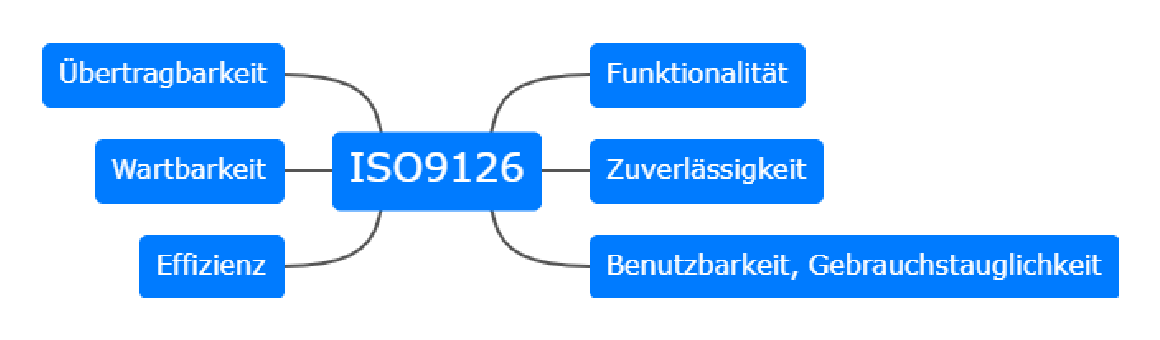
\includegraphics[width=\textwidth]{graphics/ISO-9126.pdf}
\caption[Qualitätskriterien nach ISO9126]{Qualitätskriterien nach ISO9126.\footnotemark}
\label{abb:ISO9126}
\end{figure}
\footnotetext{Mit Änderungen entnommen aus: \cite{Johner.2018}}


\pagebreak

\anhang{AWS Well Architected Referenzarchitekturen}
Folgend sind die Referenzarchitekturen aus dem \ac{AWS} Well Architected Framework - Analyticss Lens abgebildet.
\begin{figure}[H]
\centering
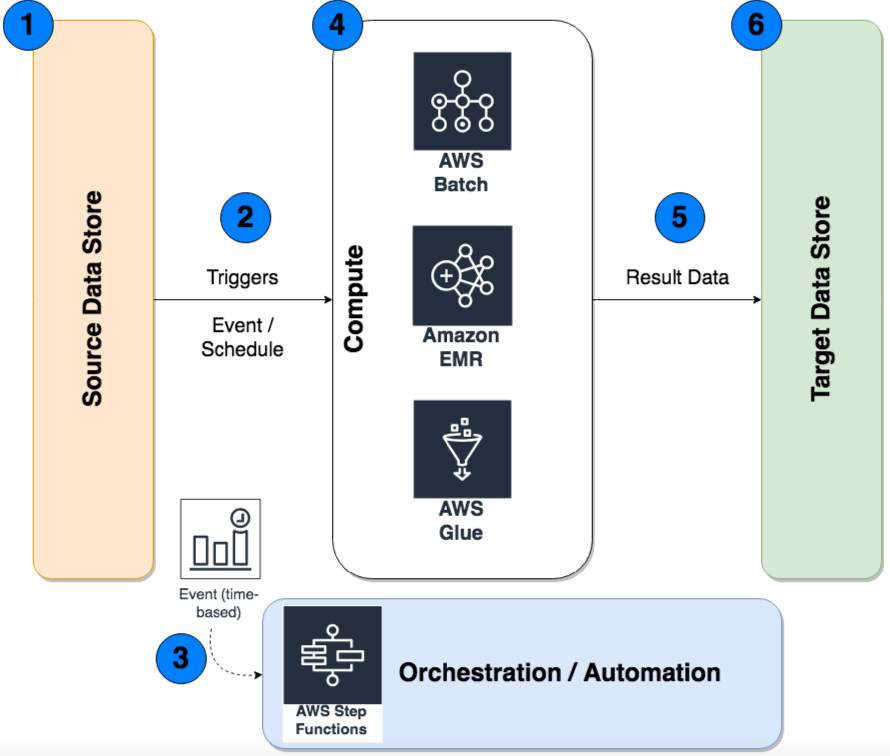
\includegraphics[width=\textwidth]{graphics/AWS-Batch-Architecture.pdf}
\caption[AWS Well Architected Batch Architektur]{AWS Well Architected Batch Architektur.\footnotemark}
\label{abb:AWSWellArchitectedBatch}
\end{figure}
\footnotetext{Entnommen aus: \cite[][12]{Ravirala.2020}}

\begin{figure}[H]
\centering
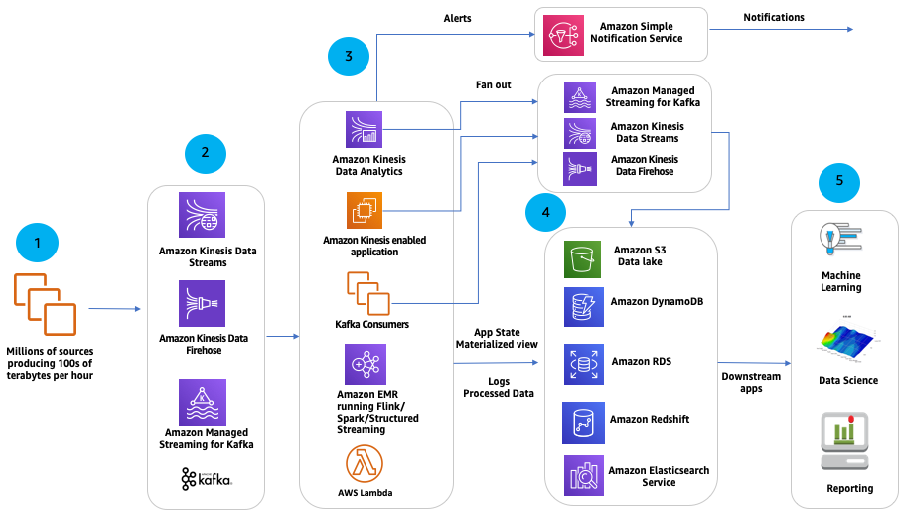
\includegraphics[width=0.92\textheight,angle=90,origin=c]{graphics/AWS-Stream-Architecture.pdf}
\caption[AWS Well Architected Stream/$\kappa$ Architektur]{AWS Well Architected Stream/$\kappa$ Architektur.\footnotemark}
\label{abb:AWSWellArchitectedStream}
\end{figure}
\footnotetext{Entnommen aus: \cite[][15]{Ravirala.2020}}

\begin{figure}[H]
\centering
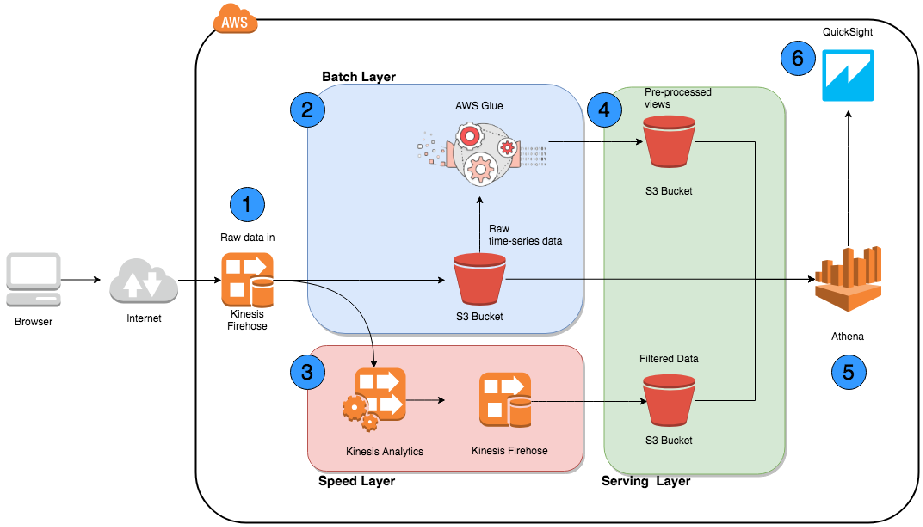
\includegraphics[width=0.92\textheight,angle=90,origin=c]{graphics/AWS-Lambda-Architecture.pdf}
\caption[AWS Well Architected $\lambda$ Architektur]{AWS Well Architected $\lambda$ Architektur.\footnotemark}
\label{abb:AWSWellArchitectedLambda}
\end{figure}
\footnotetext{Entnommen aus: \cite[][18]{Ravirala.2020}}

\anhang{Berechnungsskript Dateigröße}\label{anhang:berechnung}
Angefügt ist das verwendete Berechnungsskript für die Dateigröße, geschrieben in JavaScript, ausführbar mit der Node.JS Umgebung.

\begin{listing}[H]
\inputminted[frame=lines,breaklines=true]{javascript}{code/estimates/estimate.js}
\caption{Berechnungsskript Dateigröße}
\label{listing:js}
\end{listing}






% \anhangteil{Wieder mal eine Abbildung}\label{anhang:abbildung}
% \begin{figure}[htb]
% \centering
% 
\includegraphics[width=0.9\linewidth]{graphics/dhbw.png}
% \caption{Mal wieder das DHBW-Logo.}
% \end{figure}

% \anhangteil{Etwas Source Code}\label{anhang:sourcecode}
% \lstinputlisting{includes/HelloWorld.java}

